\documentclass[a4paper,12pt]{article}
\usepackage{amsmath}
\usepackage[margin=0.9in]{geometry}
\usepackage{braket}
\usepackage{graphicx}
\begin{document}
\subsection*{Exercise 11.1}
For a fair coin $H(X)=-2\times\frac{1}{2}\log{\frac{1}{2}}=1$\\
For a fair die $H(X)=-6\times\frac{1}{6}\log{\frac{1}{6}}=1+\log{3}$\\
For an unfair coin we can write $H(X)=-p\log{p}-(1-p)\log{(1-p)}$ and 
for the unfair die $H(X)=-p_1\log{p_1}-p_2\log{p_2}-p_3\log{p_3}-p_4\log{p_4}-p_5\log{p_5}
-(1-p_1-p_2-p_3-p_4-p_5)\log{(1-p_1-p_2-p_3-p_4-p_5)}$.\\
Differentiating both of these we see that for both the global maxima is when 
all the probabilities are equal, therefore for the unfair coin and die the entropy will
decrease.
\subsection*{Exercise 11.2}
$I(p)=k\log{p}$ is a function of probability alone.\\
$\log{p}$ is smooth for $0<p\leq 1$\\
$I(pq)=k\log{(pq)}=k(\log{p}+\log{q})=I(p)+I(q)$
\subsection*{Exercise 11.3}
$H_{bin}(p)=-p\log{p}-(1-p)\log{(1-p)}$\\
$\displaystyle \frac{dH_{bin}}{dp}=-\frac{1}{\ln{2}}-\log{p}+\frac{1}{\ln{2}}+\log{(1-p)}=0$\\
$\displaystyle\frac{1-p}{p}=1$\\
Therefore, $p=\frac{1}{2}$.
\subsection*{Exercise 11.4}
For a function $f(x)$ to be concave we require $f^{\prime\prime}(x)<0$.\\
$\displaystyle \frac{d^2H_{bin}}{dp^2}=\frac{d}{dp}(\log{(1-p)}-\log{p})=
\frac{1}{\ln{2}(1-p)p}<0$\\
Hence, $H_{bin}$ is concave.
\subsection*{Exercise 11.5}
$H(p(x,y)||p(x)p(y))=\displaystyle\sum_{xy}p(x,y)\log{\frac{p(x,y)}{p(x)p(y)}}=
\sum_{xy}p(x,y)\log{p(x,y)}-\sum_{xy}p(x,y)\log{p(x)}-\sum_{xy}p(x,y)\log{p(y)}=
\sum_{xy}p(x,y)\log{p(x,y)}-\sum_{x}p(x)\log{p(x)}-\sum_{y}p(y)\log{p(y)}=
H(p(x))+H(p(y))-H(p(x,y))$\\
$H(p(x,y)||p(x)p(y))\geq 0$\\
Therefore,\\
$H(p(x))+H(p(y))-H(p(x,y))=H(X)+H(Y)-H(X,Y)\geq 0$\\
$H(X,Y)\leq H(X)+H(Y)$\\
If $X$ and $Y$ are independent then $p(x,y)=p(x)p(y)$. Therefore,\\
$H(X,Y)=-\displaystyle\sum_{xy}p(x,y)\log{p(x,y)}=
-\sum_{xy}p(x)p(y)\log{p(x)p(y)}=-\sum_{x}p(x)\log{p(x)}-\sum_{y}p(y)\log{p(y)}=H(X)+H(Y)$\\
Therefore, equality hold if and only if $X$ and $Y$ are independent.
\subsection*{Exercise 11.6}
$H(X,Y,Z)=-\displaystyle\sum_{xyz}p(x,y,z)\log{p(x,y,z)}=
-\sum_{xyz}p(x,y,z)\log{p(x|y,z)p(y,z)}=H(Y,Z)-\sum_{xyz}p(x,y,z)\log{p(x|y,z)}$\\
$H(X,Y)-H(Y)=H(X|Y)=-\displaystyle\sum_{xy}p(x,y)\log{p(x|y)}$\\
Then, using $\log{x}\leq (x-1)/\ln{2}$ we have,\\
$H(X,Y,Z)-H(Y,Z)-H(X,Y)+H(Y)=-\displaystyle\sum_{xyz}p(x,y,z)\log{p(x|y,z)}+\sum_{xyz}p(x,y,z)\log{p(x|y)}=
\sum_{xyz}p(x,y,z)\log{\frac{p(x|y)}{p(x|y,z)}}\leq \frac{1}{\ln{2}}\sum_{xyz}p(x,y,z)\left(
\frac{p(x|y)}{p(x|y,z)}-1\right)=\frac{1}{\ln{2}}\sum_{xyz}(p(x|y)p(y,z)-p(x,y,z))=
\frac{1}{\ln{2}}\left(\sum_{xy}p(x|y)p(y)-1\right)=
\frac{1}{\ln{2}}\left(\sum_{xy}p(x,y)-1\right)=\frac{1}{\ln{2}}(1-1)=0$\\
Hence,\\
$H(X,Y,Z)-H(Y,Z)\leq H(X,Y)-H(Y)$\\
with equality when $p(x|y,z)=p(x,y)$ which is the definition for a $Z\rightarrow Y\rightarrow X$
Markov chain.
\subsection*{Exercise 11.7}
$H(Y|X)=H(Y)-H(Y:X)=-\displaystyle\sum_yp(y)\log{p(y)}-
\sum_{xy}p(x,y)\log{\frac{p(x,y)}{p(x)p(y)}}=
-\sum_{xy}p(x,y)\log{p(y)}-\sum_{xy}p(x,y)\log{\frac{p(x,y)}{p(x)p(y)}}
=\sum_{xy}p(x,y)\log{\frac{p(x,y)}{p(x)}}=-H(p(x,y)||p(x))\geq 0$\\
Equality when $p(x,y)=p(x)$, therefore when $Y$ is a function of $X$, $Y=f(X)$.
\subsection*{Exercise 11.8}
For $p(x,y,z)$ we have
$p(0,0,0)=p(0,1,1)=p(1,0,1)=p(1,1,0)=\frac{1}{4}$ and $0$ otherwise. Hence,\\
$H(X,Y,Z)=-4\frac{1}{4}\log{\frac{1}{4}}=2$\\
$H(X,Y)=H(X,Z)=H(Y,Z)=-4\frac{1}{4}\log{\frac{1}{4}}=2$\\
$H(X)=H(Y)=H(Z)=-2\frac{1}{2}\log{\frac{1}{2}}=1$\\
Therefore,\\
$H(X,Y:Z)=H(X,Y)+H(Z)-H(X,Y,Z)=1$\\
$H(X:Z)=H(Y:Z)=H(Y)+H(Z)-H(Y,Z)=0$
\subsection*{Exercise 11.9}
For $p(x_1,x_2,y_1,y_2)$ we have $p(0,0,0,0)=p(1,1,1,1)=1/2$ and $0$ otherwise. Hence,\\
$H(X_1,X_2,Y_1,Y_2)=H(X_1,X_2)=H(X_1,Y_1)=H(X_2,Y_2)=H(Y_1,Y_2)=H(X_1)=H(X_2)=H(Y_1)=H(Y_2)=
-2\frac{1}{2}\log{\frac{1}{2}}=1$\\
Therefore,\\
$H(X_1:Y_1)+H(X_2:Y_2)=2H(X_1:Y_1)=2(H(X_1)+H(Y_1)-H(X_1,Y_1))=2$\\
$H(X_1,X_2:Y_1,Y_2)=H(X_1,X_2)+H(Y_1,Y_2)-H(X_1,X_2,Y_1,Y_2)=1$
\subsection*{Exercise 11.10}
If $X\rightarrow Y\rightarrow Z$ is a Markov chain then,\\
$p(Z|Y,X)=p(Z|Y)$\\
Using $p(X|Y)=\frac{p(X,Y)}{p(Y)}$ on both sides,\\
$\displaystyle\frac{p(Z,Y,X)}{p(Y,X)}=\frac{p(Z,Y)}{p(Y)}$\\
$\displaystyle\frac{p(Z,Y,X)}{p(Z,Y)}=\frac{p(Y,X)}{p(Y)}$\\
$p(X|Y,Z)=p(X|Y)$\\
Therefore, $Z\rightarrow Y\rightarrow X$ is also a Markov chain.
\subsection*{Exercise 11.11}
$\rho=\begin{bmatrix}
    1&0\\
    0&0
\end{bmatrix}\\
S(\rho)=-1\log{1}=0$\\
$\rho=\frac{1}{2}\begin{bmatrix}
    1&1\\
    1&1
\end{bmatrix}\\
\lambda= 1$ or $0$\\
$S(\rho)=-1\log{1}=0$\\
$\rho=\frac{1}{3}\begin{bmatrix}
    2&1\\
    1&1
\end{bmatrix}\\
\lambda= \frac{1}{2}\pm\frac{\sqrt{5}}{6}$\\
$S(\rho)=-(\frac{1}{2}+\frac{\sqrt{5}}{6})\log{(\frac{1}{2}+\frac{\sqrt{5}}{6})}
-(\frac{1}{2}-\frac{\sqrt{5}}{6})\log{(\frac{1}{2}-\frac{\sqrt{5}}{6})}\approx 0.55$\\
\subsection*{Exercise 11.12}
$\rho=\frac{1}{2}\begin{bmatrix}
    1+p&1-p\\
    1-p&1-p
\end{bmatrix}$\\
$\lambda = \frac{1}{2}\pm\frac{1}{2}\sqrt{1-2p(1-p)}$\\
$S(\rho)=-\frac{1}{2}((1+\sqrt{1-2p(1-p)})\log{\frac{1}{2}(1+\sqrt{1-2p(1-p)})}\\
+(1-\sqrt{1-2p(1-p)})\log{\frac{1}{2}(1-\sqrt{1-2p(1-p)})})$\\
$H(p,1-p)=-p\log{p}-(1-p)\log{(1-p)}$\\
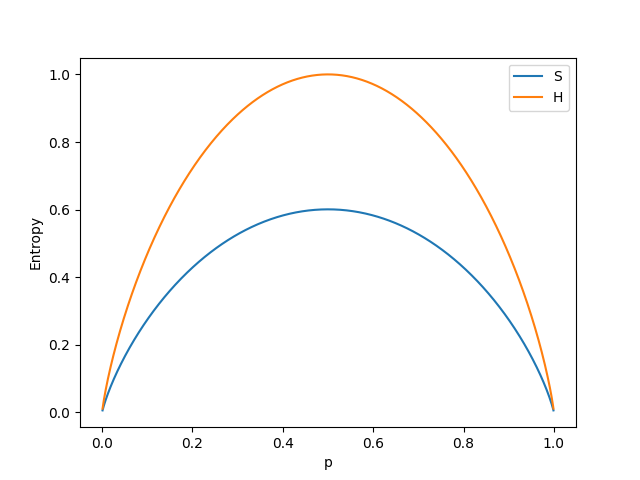
\includegraphics[scale=0.5]{12.png}\\
Therefore, $S(\rho)\leq H(p,1-p)$.
\subsection*{Exercise 11.13}
First note that for $\rho=\displaystyle\sum_i p_i\ket{i}\bra{i}$, 
$H(p_i)=\displaystyle -\sum_ip_i\log{p_i}=S(\rho)$. Then using the joint entropy
theorem for $\rho_i=\sigma$ $\forall i$ we have,\\
$S(\rho\otimes \sigma)=S(\displaystyle\sum_ip_i\rho\ket{i}\bra{i}\otimes \sigma)=
H(p_i)+\sum_ip_iS(\sigma)=S(\rho)+S(\sigma)$\\
Otherwise from the definition of the entropy for 
$\rho=\displaystyle\sum_i p_i\ket{i}\bra{i}$ and
$\sigma=\displaystyle\sum_j q_i\ket{j}\bra{j}$ we have,\\
$S(\rho\otimes \sigma)=S\left(\displaystyle\sum_{ij}p_iq_j\ket{i}\ket{j}\bra{i}\bra{j}\right)=
-\sum_{ij}p_iq_j\log{p_iq_j}=-\sum_ip_i\log{p_i}-\sum_jq_j\log{q_j}=S(\rho)+S(\sigma)$
\subsection*{Exercise 11.14}
If $\ket{AB}$ is a pure state of the composite system then $\ket{A}$ is a pure state
if and only if there's no entanglement. Hence, $S(A)\neq 0$ if and only if $\ket{AB}$ is
entangled. As $\ket{AB}$ is a pure state $S(A,B)=0$, and therefore
$S(B|A)=-S(A)$. As $S(A)\geq 0$, $S(B|A)<0$ if and only if $\ket{AB}$ is entangled.
\subsection*{Exercise 11.15}
Let $\rho=\displaystyle{I+r.\sigma}{2}$. Then\\
$\rho^\prime=M_1\rho M_1^\dagger +M_2\rho M_2^\dagger=\displaystyle
\frac{1+r_z}{2}\ket{0}\bra{0}+\frac{1-r_z}{2}\ket{0}\bra{0}=\ket{0}\bra{0}$\\
Hence,\\
$S(\rho^\prime)=-\log{1}=0$\\
Therefore, $S(\rho)\geq S(\rho^\prime)$.
\subsection*{Exercise 11.16}
$\rho^{AB}$ is a mixed state, hence\\
$\rho^A=\displaystyle\sum_i\lambda_i\rho_i^A$ and
$\rho^B=\displaystyle\sum_i\lambda_j\rho_i^B$\\
Introduce purification $R$ of $AB$\\
$\ket{ABR}=\displaystyle\sum_i\sqrt{\lambda_i}\ket{i}\ket{i^R}$\\
$\rho^{ABR}=\displaystyle\sum_{ij}\sqrt{\lambda_i\lambda_j}\ket{i}\bra{j}\otimes\ket{i^R}\bra{j^R}$\\
$\rho^R=\displaystyle\sum_{i}\lambda_i\ket{i}\bra{i}$\\
Trace over $B$,\\
$\rho^{AR}=\displaystyle\sum_{ij}\sqrt{\lambda_i\lambda_j}tr_B(\ket{i}\bra{j})\otimes\ket{i^R}\bra{j^R}$\\
Equality condition is, $\rho^{AR}=\rho^A\otimes\rho^R$, hence\\
$\displaystyle\sum_{ij}\sqrt{\lambda_i\lambda_j}tr_B(\ket{i}\bra{j})\otimes\ket{i^R}\bra{j^R}=
\sum_{ij}\lambda_i\lambda_j\rho_i^A\otimes\ket{j^R}\bra{j^R}$\\
Multiplying on both sides by $\bra{k}$ and $\ket{k}$ we get,\\
$\displaystyle\sum_{ij}\sqrt{\lambda_i\lambda_j}tr_B(\ket{i}\bra{j})\delta_{ij}=
\sum_{ij}\lambda_i\lambda_j\rho_i^A\delta_{jk}$\\
$\displaystyle\sum_{j}\lambda_j\rho_i^A=
\sum_{i}\lambda_i\lambda_k\rho_i^A$\\
$\displaystyle\sum_{ij}\lambda_i\lambda_j\rho_j^A=
\sum_{ij}\lambda_i\lambda_j\lambda_k\rho_i^A$\\
$\displaystyle\sum_{ij}\lambda_i\lambda_j(\rho_i^A-\lambda_k\rho_i^A)=0$\\
Hence, $\rho_i^A$ have a common eigenbasis.
\subsection*{Exercise 11.17}
Consider $\rho^{AB}=\frac{1}{2}(\ket{10}\bra{10}+\ket{11}\bra{11})$. Then,\\
$\rho^A=\ket{1}\bra{1}$\\
$\rho^B=\frac{1}{2}(\ket{0}\bra{0}+\ket{1}\bra{1})$\\
Therefore, $S(A,B)=S(B)=1$ and $S(A)=0$, i.e $S(A,B)=S(B)-S(A)$.
\subsection*{Exercise 11.18}
The equality condition is the same as for subadditivity inequality, i.e. $\rho^{AB}=\rho^A\otimes \rho^B$.
Hence we have,\\
$\displaystyle\sum_ip_i\rho_i\otimes\ket{i}\bra{i}=\sum_{ij}p_ip_j\rho_i\otimes\ket{j}\bra{j}$\\
Multiplying on both sides by $\bra{k}$ and $\ket{k}$ we get,\\
$\displaystyle\sum_ip_i\rho_i\delta_{ik}=\sum_{ij}p_ip_j\rho_i\delta{jk}$\\
$\displaystyle p_k\rho_k=\sum_{i}p_ip_k\rho_i$\\
$\displaystyle\rho_k=\sum_{i}p_i\rho_i$\\
$\displaystyle\sum_ip_i(\rho_k-\rho_i)=0$\\
Hence, we have equality if and only if $\rho_k=\rho_i$ $\forall i$. However, 
as this is true $\forall k$ we conclude that we have equality if and only if all
the $\rho_i$ are equal.
\subsection*{Exercise 11.19}
Consider the case of $A$ being a 2x2 matrix. Let $p_i=\frac{1}{4}$, $U_i={I,X,Y,Z}$ and
$A=c_1I+c_2X+c_2Y+c_4Z$. Hence, $tr(A)=2c_1$ as $X,Y,Z$ are traceless. Then,\\
$\displaystyle\frac{1}{4}\sum_iU_iAU_i^\dagger=\frac{1}{4}(4c_1I)=2tr(A)\frac{I}{4}=
tr(A)\frac{I}{2}$\\
We can expand this to any matrix $dxd$ size matrix by choosing $U_i$ to be the 
Sylvester's generalized Pauli matrices with $p_i=\frac{1}{d^2}$.\\
$tr(\rho)=1$, hence\\
$S(\frac{I}{d})=S(tr(\rho)\frac{I}{d})=S(\displaystyle\sum_ip_iU_i\rho U_i^\dagger)\geq
\sum_ip_iS(U_i\rho U_i^\dagger)=\sum_ip_iS(\rho)=S(\rho)$\\
As this is true for any $\rho$, the completely mixed state is the unique state of maximal entropy.
\subsection*{Exercise 11.20}
We consider a unitary matrix $U=I-2P$. Then $P=\frac{1}{2}(I-U)$ and $Q=\frac{1}{2}(I+U)$. We get,\\
$P\rho P+Q\rho Q=\frac{1}{4}(I-U)\rho(I-U)+\frac{1}{4}(I+U)\rho(I+U)=
\frac{1}{2}\rho+\frac{1}{2}U\rho U$\\
Hence, $p=\frac{1}{2}$, $U_1=I$ and $U_2=U$.\\
We can generalize this to $n$ projectors $P_i$, by taking $U=1-2P_i$ this leads to the equality,\\
$\displaystyle\sum_iU_i\rho U_i^\dagger =\sum_i(\rho-2P_i\rho-2\rho P_i+4P_i\rho P_i)=
(n-4)\rho+4\sum_iP_i\rho P_i$\\
Hence,\\
$\rho^\prime=\displaystyle\sum_iP_i\rho P_i=\frac{1}{4}\sum_iU_i\rho U_i^\dagger +\frac{n-4}{4}\rho$\\
Therefore using concavity,\\
$S\displaystyle(\rho^\prime)=S\left(\frac{1}{4}\sum_iU_i\rho U_i^\dagger +\frac{n-4}{4}\rho\right)\geq
\frac{1}{4}\sum_iS(U_i\rho U_i^\dagger)+\frac{n-4}{4}S(\rho)=
\frac{1}{4}\sum_iS(\rho)+\frac{n-4}{4}S(\rho)=S(\rho)$
\subsection*{Exercise 11.21}
Consider density matrices $\rho=\displaystyle\sum_ip_i\ket{i}\bra{i}$ and
$\sigma=\displaystyle\sum_iq_i\ket{i}\bra{i}$. As $\ket{i}\bra{i}$ are pure states we have,\\
$H(\lambda p_i+(1-\lambda)q_i)=S(\lambda\rho+(1-\lambda)\sigma)\geq 
\lambda S(\rho)+(1-\lambda)S(\sigma)=\lambda H(p_i)+(1-\lambda)H(q_i)$
\subsection*{Exercise 11.22}
For concavity $f(\lambda x+(1-\lambda)y)\geq \lambda f(x)+(1-\lambda)f(y)$ $\forall \lambda\in[0,1],p,q$.\\
Let $\lambda=\frac{1}{2}$, $x=p-h$ and $y=p+h$. Then\\ 
$f(p)\geq \frac{1}{2}(f(p-h)+f(p+h))$\\
$\frac{1}{h}(f(p-h)-2f(p)+f(p+h))\leq 0$\\
Taking the limit as $h$ goes to zero gives,\\
$f^{\prime\prime}(p)\leq 0$\\
We can write $\rho=\displaystyle\sum_ip_i\rho_i$ and
$\sigma=\displaystyle\sum_iq_i\sigma_i$
$f^{\prime\prime}(p)=\displaystyle -\sum_i\frac{(p_i-q_i)^2}{p_ip+(1-p)q_i}\leq 0$
\subsection*{Exercise 11.23}
Fix $B$. Then,\\
$f(\lambda A_1+(1-\lambda )A_2,\lambda B_1+(1-\lambda )B_ 2)=q(\lambda A_1+(1-\lambda )A_2)\geq
\lambda f(A_1,B_1)+(1-\lambda)f(A_2,B_2)=\lambda q(A_1)+(1-\lambda)q(A_2)$\\
Consider $f(x,y)=y\log{x}$, both $y$ and $\log{x}$ are concave. If $f(x,y)$ is concave then
the function $f(x,x)$ should also be concave.\\
$f(x,x)=x\log{x}$, however $f^{\prime\prime}=\frac{1}{x}\geq 0$, hence it's not concave.
Therefore we have a contradiction and $f(x,y)$ is not jointly concave.
\subsection*{Exercise 11.24}
Let $R$ be the purification for the system $ABC$. Then from strong subadditivity,\\
$S(R,B,C)+S(B)\leq S(R,B)+S(B,C)$,\\
however $S(R,B,C)=S(A)$ and $S(R,B)=S(A,C)$, therefore\\
$S(A)+S(B)\leq S(A,C)+S(B,C)$
\subsection*{Exercise 11.25}
Consider the state $\lambda \rho\otimes \ket{0}\bra{0}+(1-\lambda)\sigma \otimes\ket{1}\bra{1}$,
where $\rho$ and $\sigma$ are density matrices of the system $AB$ and the rest of system $C$.
Then by the strong subadditivity inequality, equation (11.57), exercise 11.13  and using $S(A|B)=S(A,B)-S(B)$ we get,\\
$S(A|B)_{\lambda\rho+(1-\lambda)\sigma}\geq S(A,B,C)-S(B,C)=S(A,B,C)-S(A)=H(\lambda)+\lambda S(\rho\otimes \ket{0}\bra{0})+
(1-\lambda)S(\sigma\otimes \ket{1}{1})-H(\lambda)-\lambda S(tr_B(\rho))-(1-\lambda)S(tr_B(\sigma))=
\lambda (S(\rho)-S(tr_B(\rho)))+(1-\lambda)(S(\sigma)-S(tr_B(\sigma)))=
\lambda S(A|B)_\rho+(1-\lambda)S(A|B)_\sigma$\\
As this is true for all $\lambda$, $\rho$ and $\sigma$, $S(A|B)$ is concave.
\subsection*{Exercise 11.26}
Using, $S(B)+S(C)\leq S(A,B)+S(A,C)$,\\
$S(A:B)+S(A:C)=S(A)+S(B)-S(A,B)+S(A)+S(C)-S(A,C)\leq 2S(A)+S(B)+S(C)-S(B)-S(C)=2S(A)$\\
Consider $\ket{AB}=\frac{1}{\sqrt{2}}(\ket{00}+\ket{11})$,\\
$S(A,B)=0$, $S(A)=S(B)=1$. Hence, $S(A:B)=2>S(A)$.
\end{document}